\documentclass[10pt,a4paper]{article}

\usepackage{afterpage}
\usepackage{graphicx}
\usepackage{float}

\usepackage{hyperref} 
\usepackage{fontspec}
\setmainfont{GFS Artemisia}

\usepackage{geometry}
\usepackage{amssymb}
\usepackage{xcolor}
\begin{document}
\title{Parallel And Distributed Systems \\ Assignment 3}
\author{Konstantinos Chatziantoniou 8941}
\date{20/1/2019}
\maketitle


\section*{Intro}
In this assignment, the knn search algorithm will be parallelized, using the GPU(cuda). For the version of knn search that is used, the queries and corpus are split into blocks. The algorithm  first searches inside the block of the query (primary candidates), and if necessary expands the search to the adjacent blocks. The program is written in \textbf{Cuda/C} and benchmarks were ran on a \textbf{GTX 960 4gb} graphics card \textbf{i3 4170} CPU.
\section*{Code}
Code is available on \textcolor{violet}{\href{https://github.com/KonstantinosChatziantoniou/GridKnn-Cuda}{github}}. \\ \textit{"https://github.com/KonstantinosChatziantoniou/GridKnn-Cuda"}


\section*{Serial Algorithm}
\subsection*{Binning}
First, the data is grouped into equally sized boxes. The queries and corpus follow uniform distribution in [0,1] $\mathbb{R}^3$ , so every box will contain approximately the same amount of points. A grid of boxes is applied to the space, with dimensions $[grid\_d,grid\_d,grid\_d]$, meaning there will be $grid\_d^3$ boxes. Each side of the box has a length of $side\_length = 1/grid\_d$. Then it's calculated in which box each query and point belongs, $blockId_x = coordinate_x \% side\_length$, 
and rearranged so that the points in a particular box occupy continuous space in memory. The amount of points in each block is stored in an array.
\subsection*{KNN - Primary Candidates Search}
In order to find the nearest neighbor among the primary candidates, we iterate through every query and then iterate through every point in the current block and save the one with the least distance. \\
After, we compare the distance of the nearest neighbor to the distance of the query from the bounds of the box to determine if we have to expand the search.
\subsection*{KNN - Adjacent Boxes} 
If there is a possibility that there is a point in adjacent boxes with smaller distance the nearest neighbor from the primary candidates we have to search them too. To find the blockId of the adjacent boxes, we calculate all the possible combinations of currentBlock +1,-1,+0 and keeping those that are in bounds of the grid. Then we iterate through the queries with unconfirmed neighbor, through the adjacent boxes and through the points in them.
\subsection*{Verification}
The validation of the neighbors was done using \textbf{scikit} package in a python script, which also ran the program for different number of queries, corpus and different dimensions of the grid.


\section*{Parallel algorithm/CUDA}
We have to determine which part of the program will be parallelised. The process of "binning" has time complexity O(n). It takes less than 2 sec for $N = 2^{23}$ and $grid\_d = 2^5$, which is not significant, but 15sec for $grid\_d = 2^6$. On the other hand, the knn search takes a lot more,especially for large data sets. \\

\subsection*{Parallelisation method}
After many attempts, the most efficient approach was to parallelise based on the queries. Since each query belongs in a block, it's only logical to assign a cuda-block to space block. So, the first parameter of the execution configuration will be \textcolor{blue}{dim3}$(grid\_d,grid\_d,grid\_d)$. The next parameter is the number of threads for each block. We will set this to 1024 (max thread number per block for gtx960) for now. The threads of one block have to search the nearest neighbor among the points of the block for all the queries in the block. But there are only so many threads in the cuda-block($2^{10}$) and probably much more queries and points $2^{23-3\cdot grid\_d}$. So, the queries will be processed in group of 1024(number of threads). \\

This alone was not enough. Every thread reads every from the global memory, which is very slow (400~600 cycles).Lets call the time required to get a point from global memory 'mem-cycle'.Since the threads in each block iterate through the same points, it will be efficient to store the points to the shared memory. Now it will take one 'mem-cycle' to get 32 points from the global memory (32 is the max number of threads that can read data from the memory simultaneously). If we don't use shared memory, the gpu will spend a 'mem-cycle' for each point, 32 times more. \\ 

Also, it doesnt make sense to check whether the nearest primary candidate is the actual nearest neighbor, like we did in the serial version. If we branch out a thread, it will not be available to do other work, but wait for the warp to finish the session. Also if we 'return' the thread it might mess up the synchronisation and the writes to the shared memory.

\subsection*{Verification}
The validation of the neighbors was done using \textbf{scikit} package in a python script, which also ran the program for different number of queries, corpus and different dimensions of the grid.

\section*{Results and Comments}
\subsection*{Parallel vs Serial}
Bellow is laid out the comparison between the serial and the cuda version of knn search. Only the times of the search are shown, not the binning,data reading and printing times. 
\textit{Reminder: The maximum time of binning for up to 32 grid dimension was approximately 1s, whereas for grid dimension of 64 the binning time was 15s.}

\begin{center}
\centering
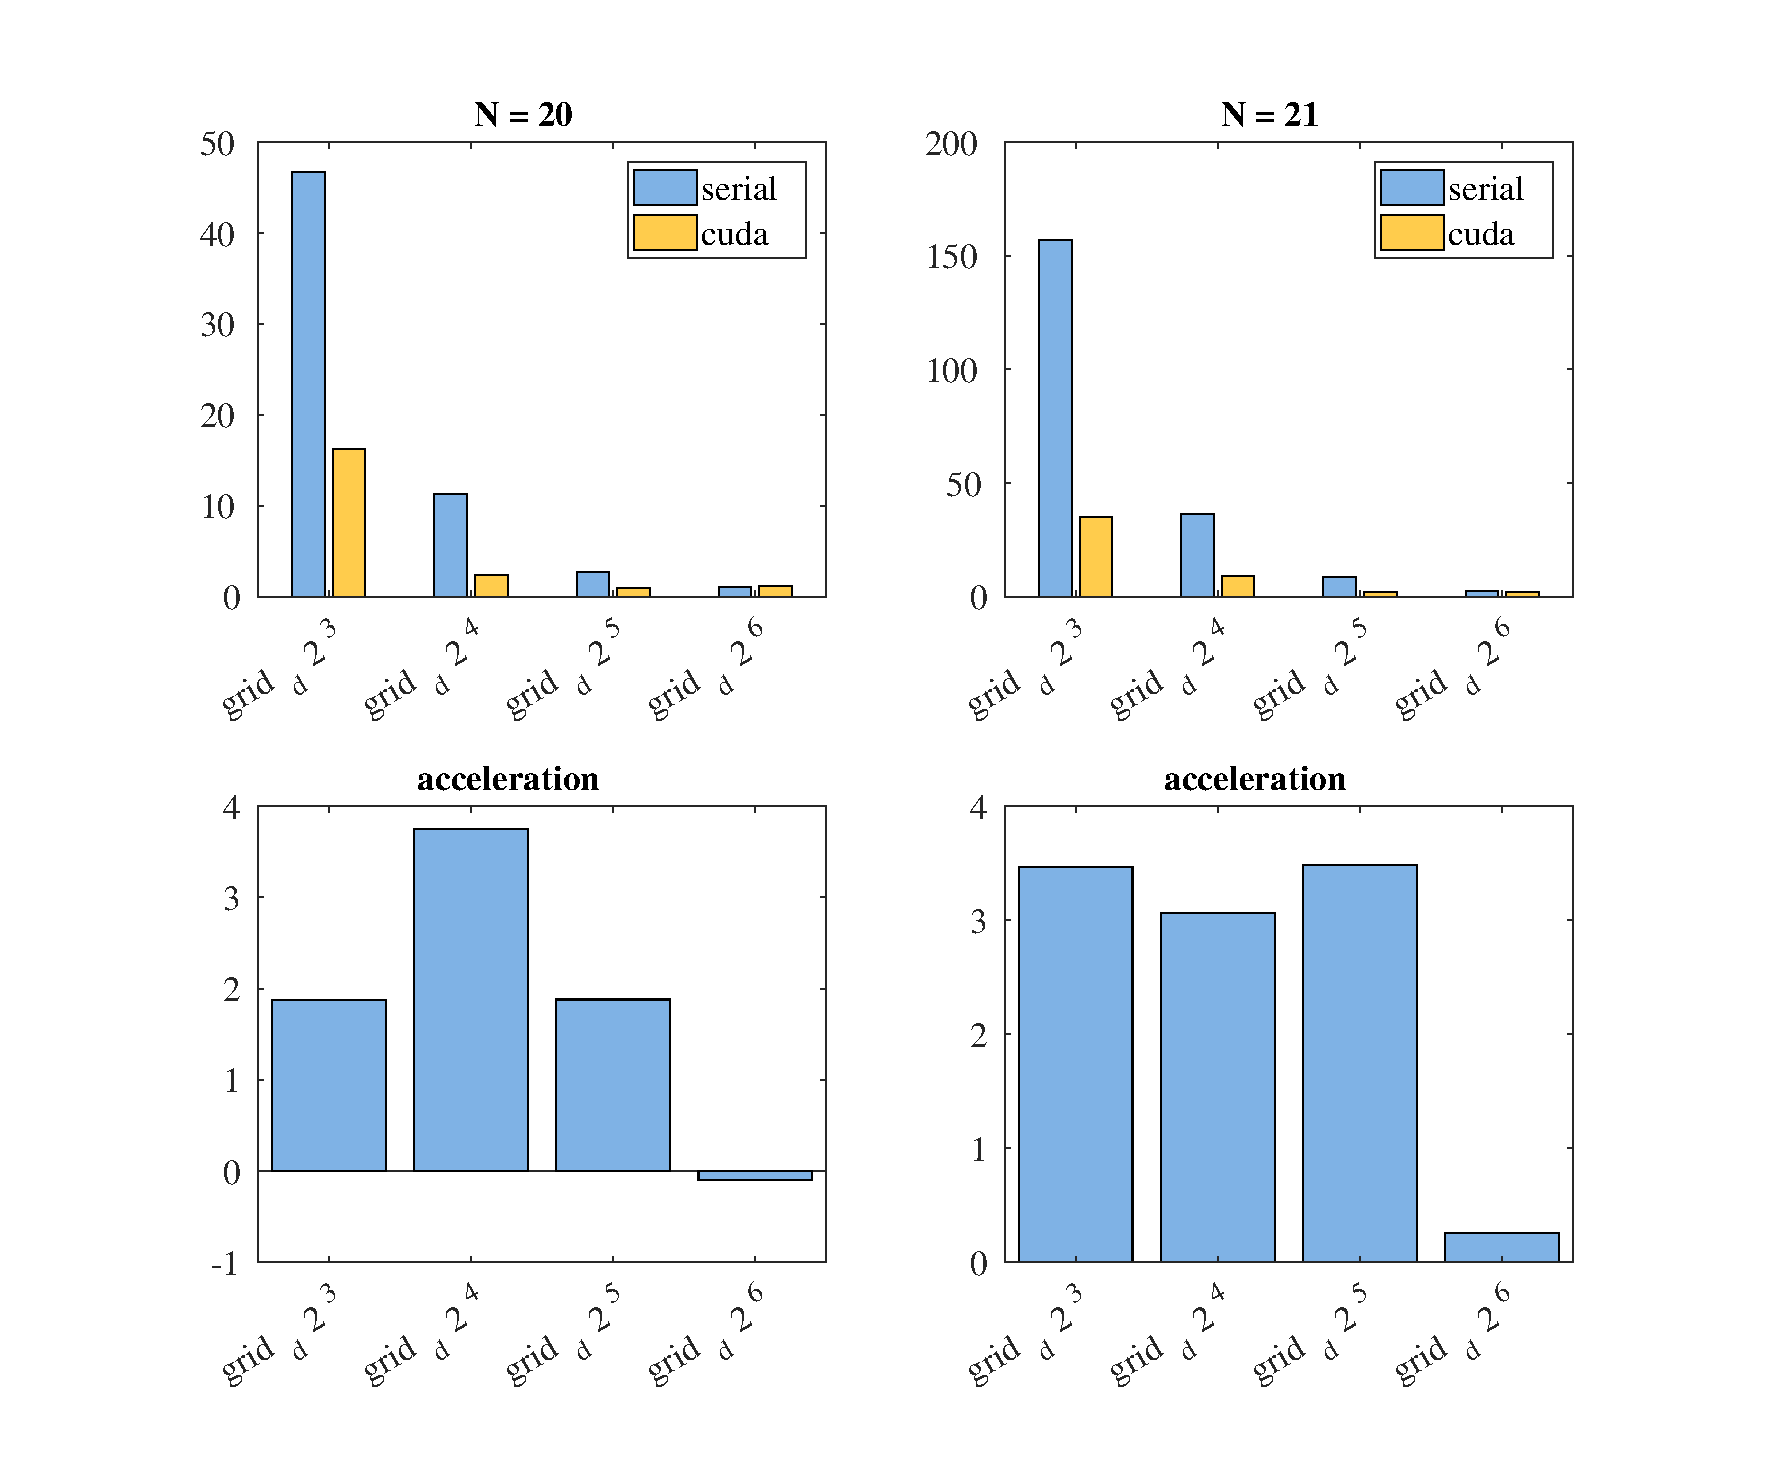
\includegraphics[scale=0.5]{cuda2021}
\end{center}

\begin{center}
\centering
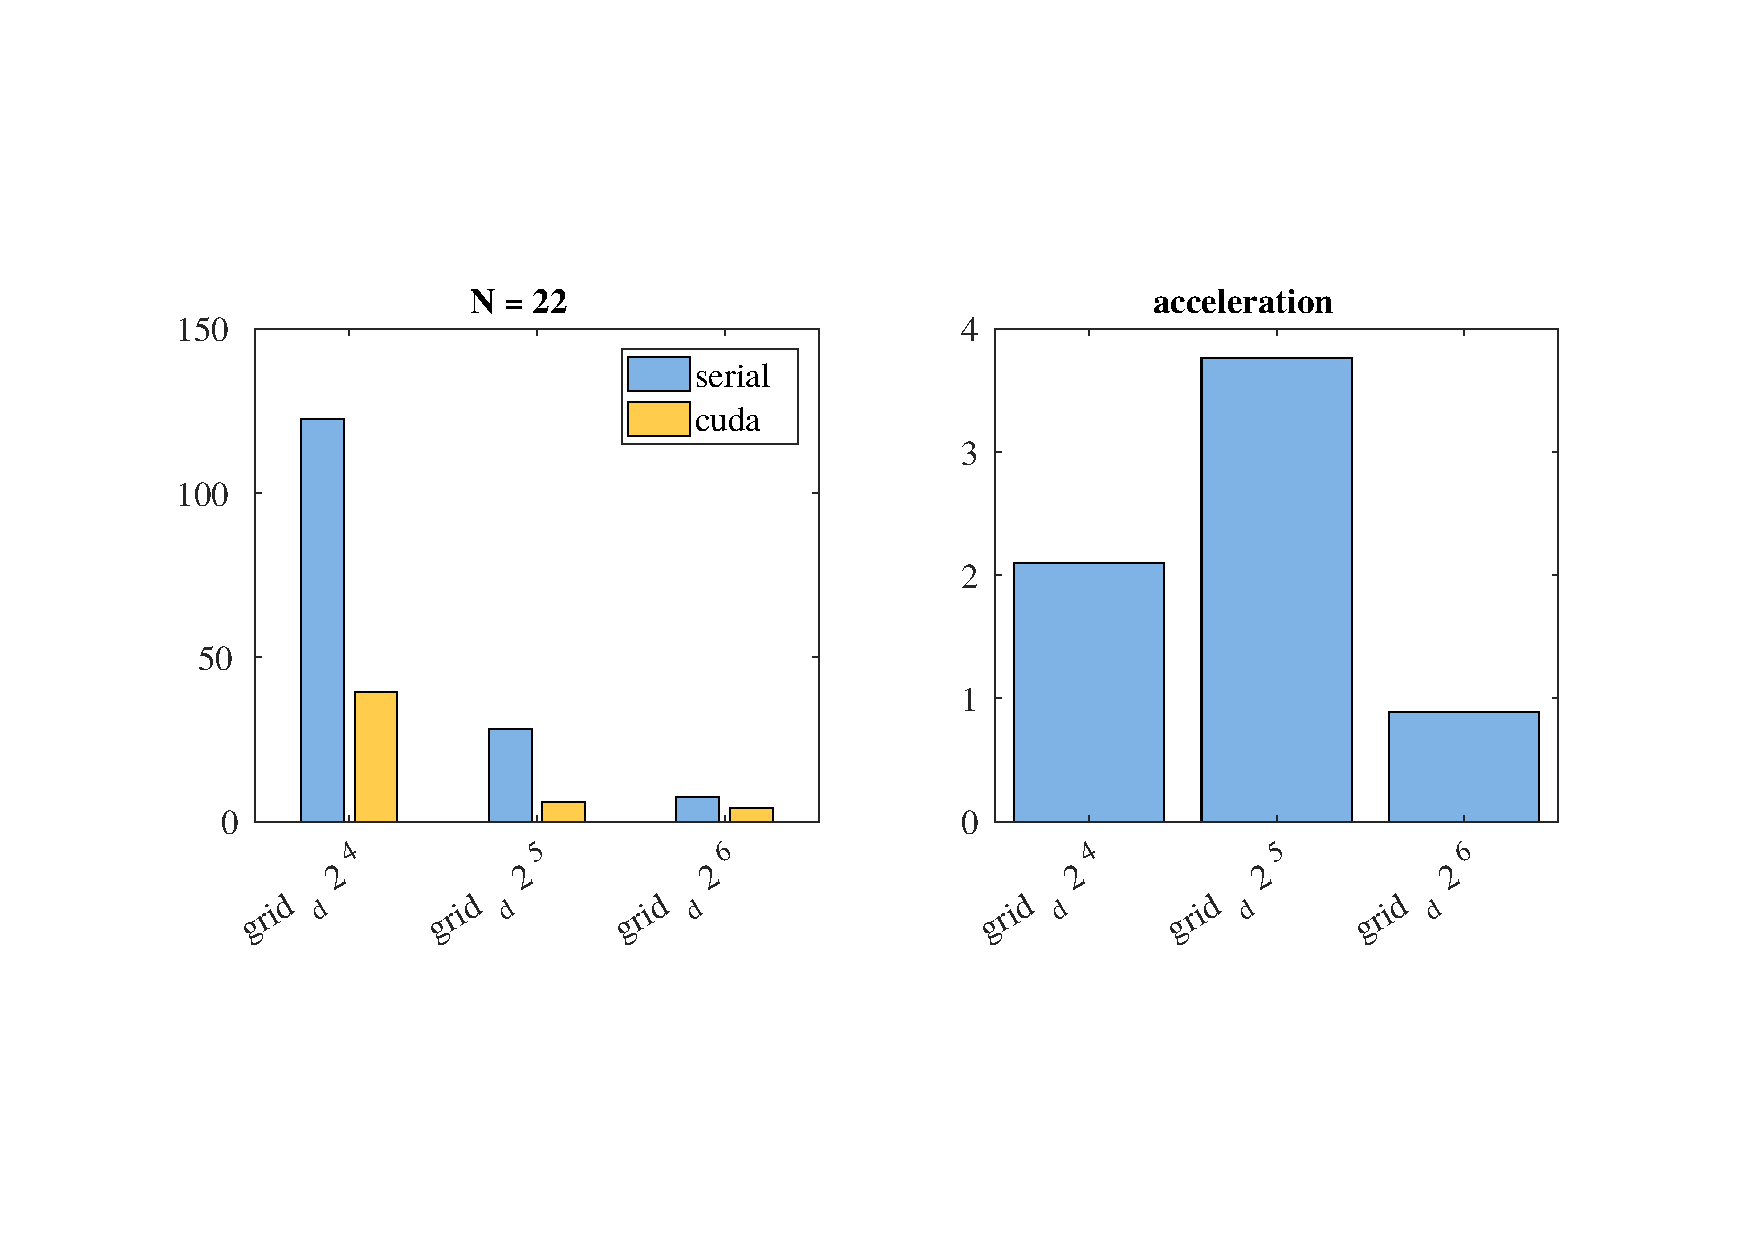
\includegraphics[scale=0.5]{output}
\end{center}

\begin{figure}
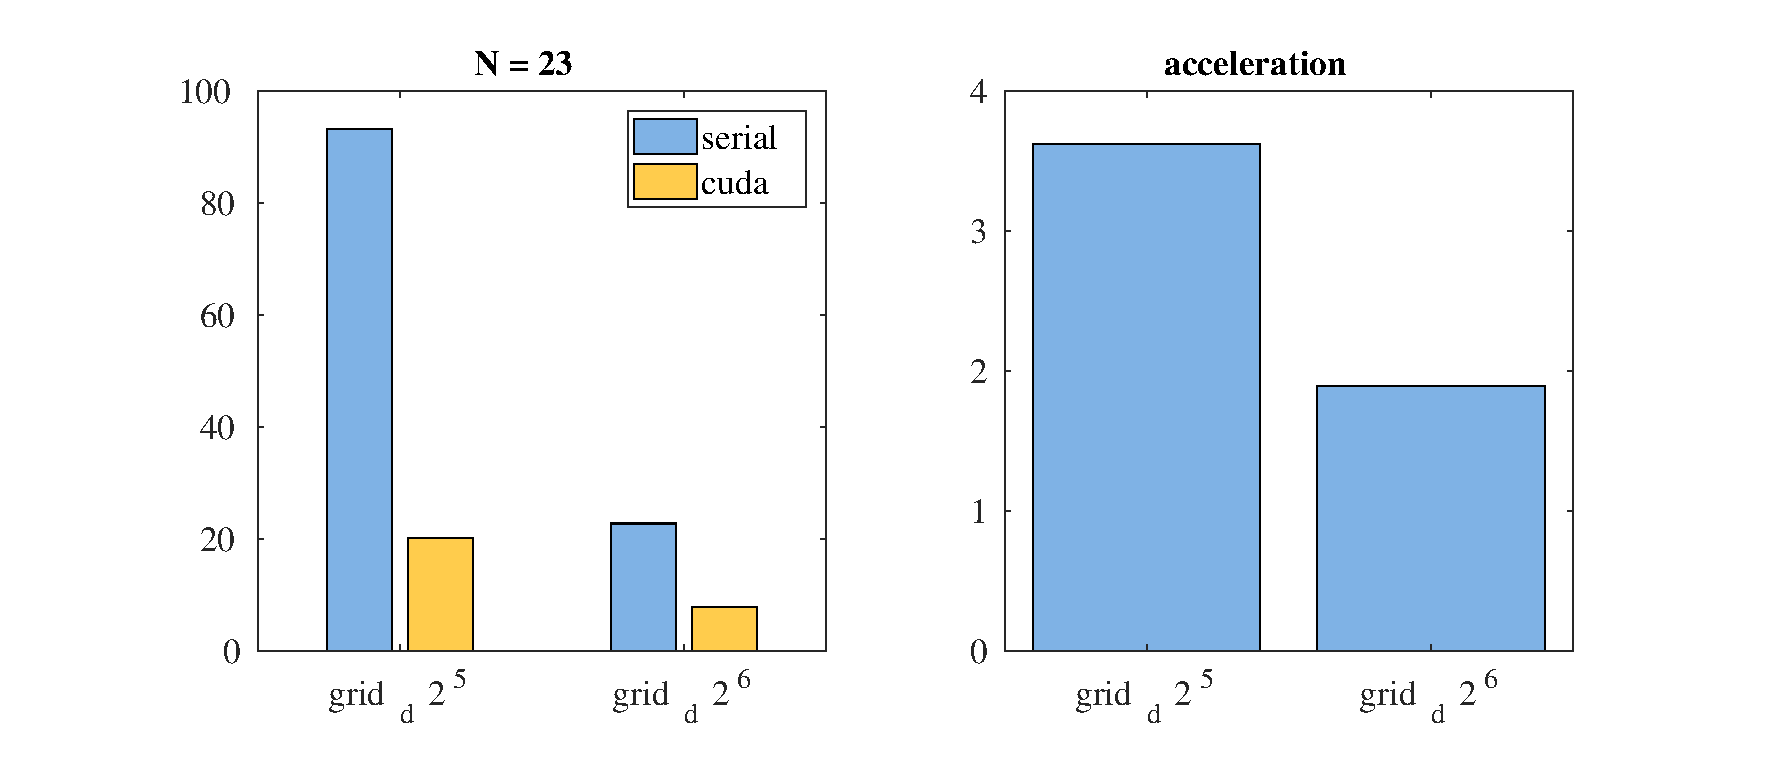
\includegraphics[scale=0.5]{cuda23}
\end{figure}

\subsubsection*{Observations}
Cuda manages to be 3-4x times faster in general, except for one case.
\begin{itemize}
\item The bigger the grid dimensions, the faster both versions run.
\item For grid dimension = 64, there is not a significant boost with cuda (for $N = 2^{20}$ it's even a little bit slower than the serial). If we also ,take into account the binning time for $grid\_d$  = 64, it seems it's not worth it using that big dimension. For the cuda version with $N=2^{23}$, for $grid\_d=32$ $search time = 20s$ and $binning time = 0.8s$ with total 20.8s, For $grid\_d = 64$ $search time = 7.8s$ and $binning time = 15.6$ with total 23.4s.
\item Using $grid\_d = 2 and 3$ for $N \geq 2^22$ was really slow and made the system unresponsive or caused \textit{CudaLaunchTimeError}, so thew were not included in the benchmarking graphs.
\end{itemize}

\subsection*{Parallel, 1024 vs 128 threads}
Below is laid out the comparison between 2 cuda programs, one with 1024 threads per block and one with 128.

\begin{figure}[H]

\centering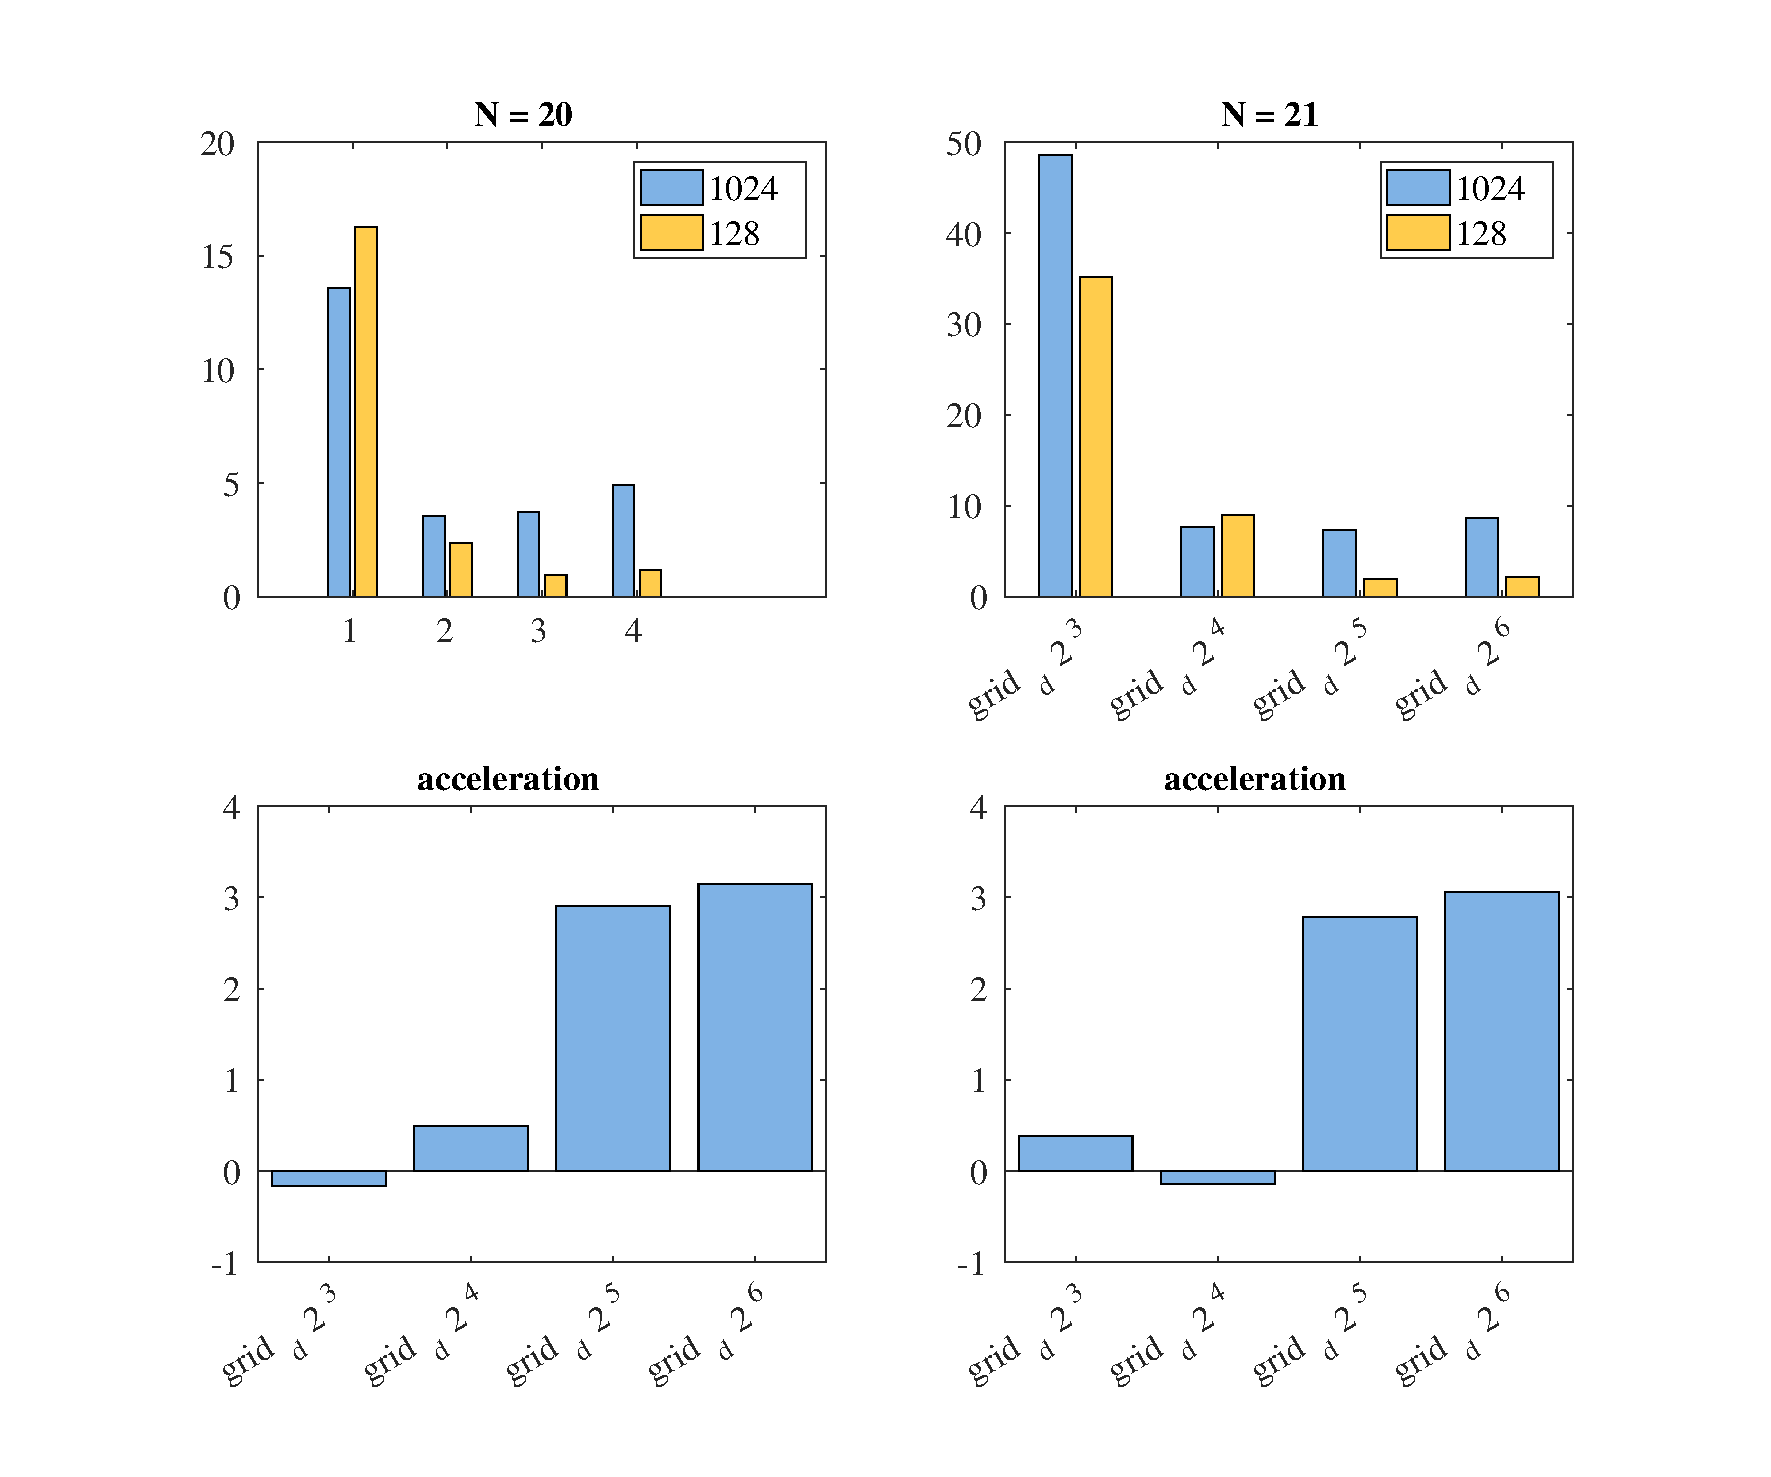
\includegraphics[scale=0.5]{threads2021}
\end{figure}

\begin{figure}[H]

\centering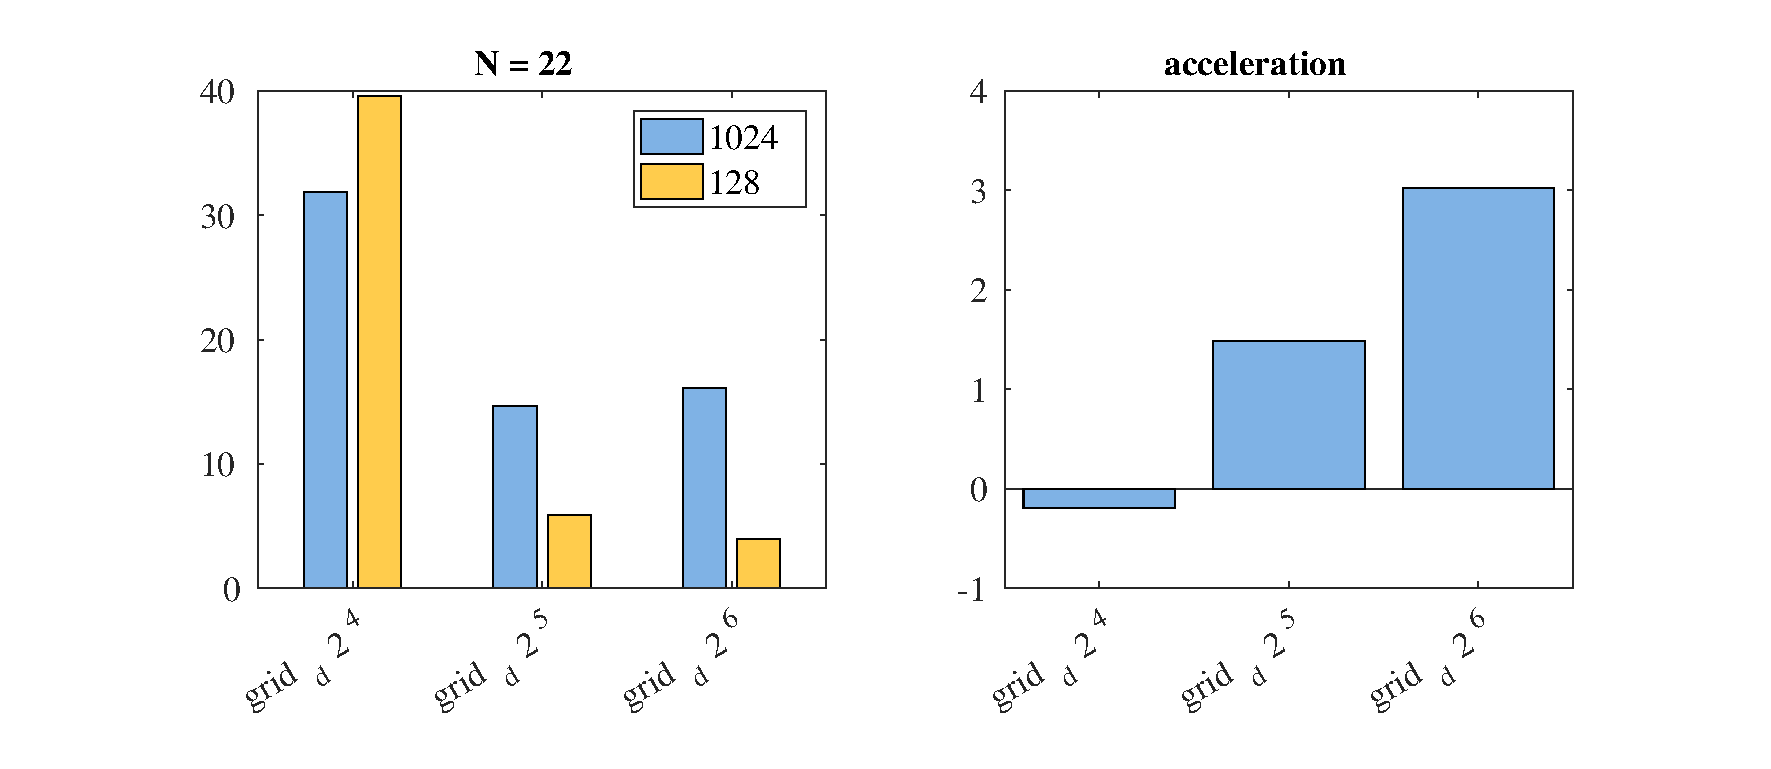
\includegraphics[scale=0.5]{threads22}
\end{figure}

\begin{figure}[H]

\centering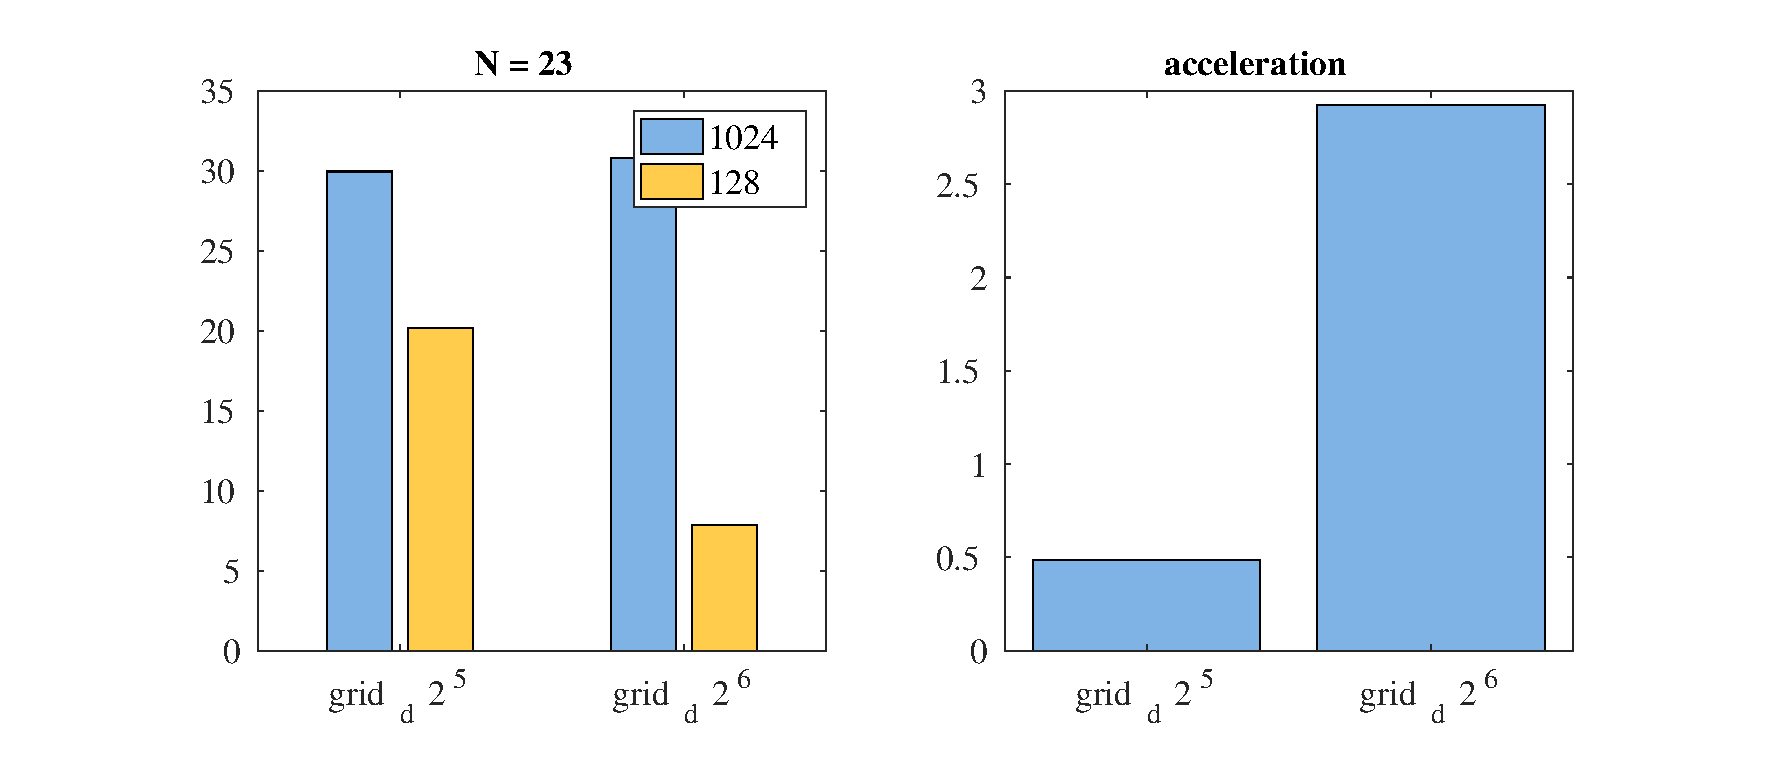
\includegraphics[scale=0.5]{threads23}
\end{figure}



It is apparent that 128 threads manage better than 1024 for big grid dimension. Lowering the threads to 128, we still take advantage of the shared memory and group reads from the global memory, and there are not as much idle threads when the blocks contain a few points ($\leq2^{6}$) for big grid dimensions.
We should also note that for 1024 threads, the search time slightly increases when we increase the grid dimension, after a certain point.


\subsubsection*{Problems}
\begin{itemize}
\item The programs produce correct results for the parameters mentioned above. We should note that for $N = 2^{20}$ and $grid\_d$ = 64, we heavily rely on the uniform distribution for correct results. If we have a perfect uniform distribution there should be only 4 points per block. Since we don't check further than the adjacent blocks, if the primary candidates are zero ,the side adjacent blocks also contain no points and the edge adjacent have points, the result might be wrong.
\item Using $grid\_d = 2 and 3$ for $N \geq 2^{22}$ was really slow and made the system unresponsive or caused \textit{CudaLaunchTimeError}, so thew were not included in the benchmarking graphs.$N \geq 2^{24}$ caused \textit{Segmentation Fault}, probably because the memory provided by the OS was not enough. The program tried to allocate more than 100mb of memory on the stack. Changing the kernel limit was not recommended.
\end{itemize}


\end{document}